\chapter{Knowledge Graph Completion}
\label{cha:knowledge_graph_completion}

As discussed in section \ref{cha:knowledge_graphs} knowledge graphs are not complete. They contain noisy  and incomplete data. It is practically impossible to cover every possible entity and relation existing in the real-world or even in their domain. There might be missing entities and relations or a Knowledge Graph can include two entities/ relations representing the same real-world entity. Knowledge graph completion tries to tackle these and other problems. It can be seen as a way of data cleaning for knowledge graphs. The solutions to the problems are defined into clear tasks, these include: entity resolution and entity and link prediction approaches. \\

\textbf{Entity Resolution} is according to Talburt "the process of determining whether two [entities] are referring to the same object or to different objects". \cite{talburt_entity_2011} \\ 

\textbf{Entity Prediction} is the task of integrating new entities into the knowledge graphs. These entities are are discovered from other external sources and the knowledge graph includes no information about them. The goal is to find all possible relations this new entity has to the entities already existing in the graph. \cite[p.~1]{baumgartner_entity_2021} \\

\textbf{Link Prediction} is quiet similar to entity prediction. Instead of finding links for a new entity the goal here is to find all missing relations between already existing entities. \cite[p.~125]{golbeck_analyzing_2013} Link prediction can be approached in two different ways: entity classification and triple classification. "Entity classification tries to predict the type or the class of an entity [...]" \cite{ilkou_symbolic_2020} For a triple with a missing tail $(h,r,?)$ the goal would be to list all entities which fit into the tail along with their confidence. Triple classification on the other hand is a binary tasks. Here the input is a compete triple $(h,r,t)$ and the goal is to predict whether this triple is true or not. \cite{ilkou_symbolic_2020} \\

In the following we are going to focus on the task of link prediction. There are various models tackling the problem. They can be categorized into one of the following two categories: symbolic and sub-symbolic approaches. Symbolic approaches are based on a high-level symbolic representation of the problem and try to reason about the problem with logic, this makes them comprehensible for humans. Sub-symbolic approaches on the other hand, solve the problem through less explainable mathematical equations. \cite{ilkou_symbolic_2020}

\section{Symbolic Approaches}
\label{cha:symbolic_methods}
Symbolic approaches, or also sometimes referred to as "Good Old Fashioned Artificial Intelligence", focus on learning hypothesises in a symbolic (logical) language. \cite{hogan_knowledge_2020} The strength of models from this approach lies in their explainability. Since the learned hypothesis are expressed in a logical language, either as axioms or rules, they are interpretable for a human and we can therefore reason about their predictions. In the following we will focus on rule-based models because they are more present for the link prediction tasks.  \cite{hatzilygeroudis_neuro-symbolic_2005} 
Rules are basically if-then clauses. Each rule has one or more conditions which have to be true and if they hold true the rule "fires" and its conclusion can be derived. They are often written down as Horn clauses, an example for a Horn clause can be seen in its disjunctive and implicative form in equation \ref{eq:horn_disjunct} and \ref{eq:horn_implic} respectively. \cite{chandra_horn_1985}

\begin{equation}
\label{eq:horn_disjunct}
A \wedge \neg B_1 \vee \neg B_2 \vee ... \vee \neg B_n \end{equation}

\begin{equation}
\label{eq:horn_implic}
A \leftarrow B_1, B_2, ..., B_n
\end{equation}

Both equations express the same clause which states that if all conditions $B$, also called body atoms, are true so is the conclusion $A$, which is also referred to as the head.

\subsection{AnyBURL}
\label{cha:anyburl}
AnyBURL \cite{meilicke_anytime_2019}, short for Anytime Bottom-Up Rule Learning, is a link prediction algorithm that generates a set of rules from an existing knowledge graphs and leverages the generated rules to make predictions. The core idea behind AnyBURL  is that "[...] sampled paths from a knowledge graph (random walks) are examples of very specific rules, which can be transformed into more general rules." \cite{ott_safran_2021} 






\subsubsection{Learning Rules}
Rules are learned bottom-up, meaning we start with a sampled random path in the knowledge graph which then gets generalized into a rule. The sampled random path is called the ground path or grounding. In \cite{meilicke_anytime_2019} generalized rules are classified into three types $AC_1$, $AC_2$ and $C$. 

$C$ rules are generalizations of cyclic 
ground paths:

\begin{equation}
h(Y,X) \leftarrow b_1(X, A_2), ..., b_n(A_n,Y).
\end{equation}

$AC_2$ rules are generalizations of acyclic ground paths:

\begin{equation}
h(c_0,X) \leftarrow b_1(X, A_1), ..., b_n(A_n,A_{n+1}).
\end{equation}
	
$AC_1$ rules can be generalized from both cyclic (with $c_0=c_{n+1}$) and acyclic ones ($c_0\neq c_{n+1}$):

\begin{equation}
h(c_0,X) \leftarrow b_1(X, A_1), ..., b_n(A_n,c_{n+1}).
\end{equation}

$X$ and $Y$ are for variables appearing in the head of the Horn clause, $A_i$ is a variable appearing only in the body and $c_i$ is a constant. Furthermore, $h(e_1,e_2)$ and $b_i(e_1,e_2)$ are another notation to express a triple $(e_1, h, e_2)$ or $(e_1, b_i, e_2)$.

\section{Sub-Symbolic Approaches}
\label{cha:sub_symbolic_methods}

Sub-symbolic approaches are based on statistics. They try to learn numerical models from the existing facts in the knowledge graph. These models can then be used to predict the existing of a triple.  \cite{nickel_review_2015} The most prominent models for knowledge graph completion of this approach are embedding-based models. These models learn a vector representation for each entity and relation. This is also often referred to as an embedding. In this representation it is then assumed that similar entities and similar relations will have similar vectors. An example for these embeddings can be seen in figure \ref{fig:embedding_example}. On the left side we see a knowledge graph with three entities and two relations. Every entity and relation are represented on the right side by an embedding. Our two entities \textit{Washington D.C} and \textit{New York City} are both cities and therefore we can assume that their semantic meaning are quiet similar. The embeddings of these two entities are also quiet similar which demonstrates that our previous assumption is correct. \cite{bianchi_knowledge_2020} Our embeddings are also called latent features because they can not be directly observed in the data. Instead our model has to infer these features from the data. \cite{nickel_review_2015} 

\begin{figure}[H]
\centering
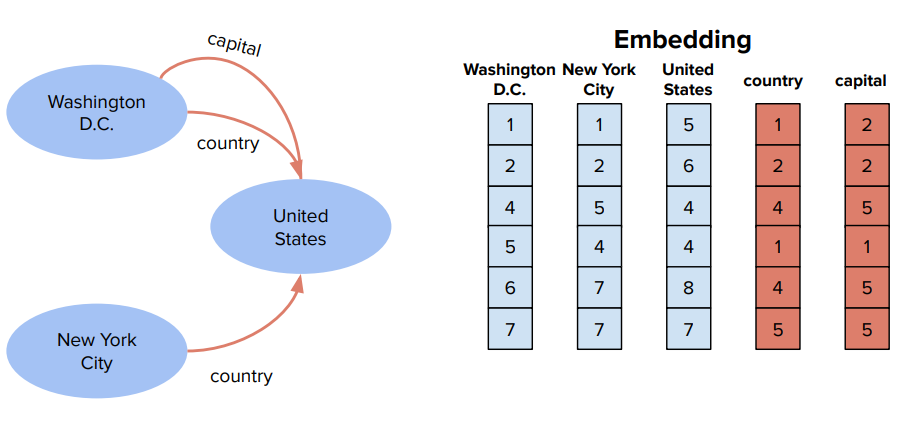
\includegraphics[width=0.9\textwidth]{images/embedding_example.png}
\caption{Example of an Embedding for a Knowledge Graph}
\label{fig:embedding_example}
\end{figure}

An embedding-based model is defined by three characteristics \cite{bianchi_knowledge_2020}:

\begin{enumerate}
\item representations of entities and relationships
\item the scoring function
\item the loss function
\end{enumerate}

As stated earlier our entities and relations are represented through vectors, their embeddings. Some models vary from this a bit and use complex numbers instead of real ones \cite{trouillon_complex_2016}  or use matrices to represent relationships \cite{nickel_three-way_2011}.
\\
The score function $f(h,r,t)$ calculates the distance between the embeddings of two entities relative to their relation. If the triple holds true, its score should be in an optimal case equal to $1$. \\
Lastly the loss function defines the objective which is going to be minimized during the training of our model where the embeddings for our entities and relations are learned.

\subsection{RESCAL}
\label{cha:rescal}
One such an embedding-based model is RESCAL \cite{nickel_three-way_2011}\cite{nickel_factorizing_2012}. The model explains triples via pairwise interactions of latent features. It calculates the score of a triple as

\begin{equation}
\label{eq:rescal_score}
s(h,r,t)=e_h^T M_r e_t
\end{equation}

where $e_h, e_t \in \mathbb{R}^D$ and $M_r \in \mathbb{R}^{D*D}$. In this formula the interactions between two entity vectors are captured using only multiplicative terms, which makes this a bilinear model.

Furthermore, we can see that entities are encoded into a $D$-dimensional vector representation and have the same representation regardless of whether they occur as head or tail entity in a triple. Moreover, they also share the same representation for entities independent of the relation in a triple. Meaning that for every relation the vector of an entity stays the same. In \cite{nickel_review_2015} the authors of the RESCAL model argue that this allows their model to "[...] propagate information between triples [...]" and "[...] capture global dependencies in the data.". The relation in equation \ref{eq:rescal_score} is represented via a matrix $M_r$. Important to note about this matrix is its asymmetry. This allows the model to capture asymmetric relations. E.g. while the model should predict the triple $(Darth\_Vader,$ $ father\_of,$ $ Luke\_Skywalker)$ as \textit{True}, the triple $(Luke\_Skywalker,$ $ father\_of,$ $ Darth\_Vader)$ should be predicted as \textit{False}. 

\subsubsection{Training through RESCAL-ALS}
The model is trained through finding estimates for the matrices $E$ and $M_r$ which can be achieved by solving following regularized minimization problem

\begin{equation}
\label{eq:rescal_min_problem}
\min_{E, M_r} f(E,M_r) + g(E, M_r)
\end{equation}

where 

\begin{equation}
\label{eq:rescal_als}
f(E,M_r)=\frac{1}{2}(\sum_{h,r,t} \norm{X_{hrt}-s(h,r,t)}^2_F)
\end{equation}

and 

\begin{equation}
\label{eq:rescal_regu}
g(E, M_r)=\frac{1}{2}\lambda(\norm{E}^2_F + \sum_k\norm{M_r}^2_F).
\end{equation}

The term $g$ is included as regularization term to prevent the model from overfitting. The regularized minimization problem in equation \ref{eq:rescal_min_problem} is solved with an for RESCAL adjusted version of the alternating least-squares approach called RESCAL-ALS. This approach consists of a sequence of very efficient, closed-form updates as described in \cite{nickel_factorizing_2012}. This training method assumes the closed-world assumption.

\subsubsection{Training through Pairwise Loss}
In \cite{nickel_review_2015} an alternative training method under the open-world assumption is presented which is more similar to the way other embedding-based models are trained. They refer to it as pairwise loss. Here two sets of triples are used to train the model, positives and negatives denoted as $D^+$ and $D^-$ respectively. The positive triples are every known existing triple in our knowledge graph and the negative triples are created by corrupting existing triples. For the triples in the negative set it is not guaranteed that they are negative since a randomly corrupted triple could actually be an unknown true fact, but they are seen as \textit{assumed-to-be-negative}.

Using stochastic gradient descent or any of its variations following objective function is then minimized 

\begin{equation}
\label{rescal_pairwise}
\min_{E,M_r} \sum_{x^+ \in D^+} \sum_{x^- \in D^-} \mathcal{L}(s(x^+), s(x^-)) + g(E, M_r)
\end{equation}

using the same regularization as in equation \ref{eq:rescal_regu} and where $\mathcal{L}$ is a margin-based ranking loss function such as

\begin{equation}
\label{eq:rescal_loss}
\mathcal{L}(s,s') = max(1+s'-s,0).
\end{equation}
 
The usage of the margin-based loss has the advantage that negative triples do not have to be necessarily negative, they just have to be "more negative" than the positive ones. 

\subsection{DistMult}
\label{cha:distmult}
DistMult \cite{yang_embedding_2015} is another embedding-based model. It also uses the same basic bilinear scoring function as RESCAL in equation \ref{eq:rescal_score}. The difference here is that DistMult restricts the relation matrix $M_r$ to be a diagonal matrix. This reduces the parameters for the learnable parameters for a single relation from $D*D$ to just $D$. Therefore DistMult can be seen as a simplified version of RESCAL with the score function

\begin{equation}
\label{eq:distmult_score}
s(h,r,t)=e_h^T diag(r) e_t
\end{equation}

where $e_h, e_t$ and $r\in \mathbb{R}^D$. The reduction of the relation dimensionality makes the model more computational efficient, especially on large knowledge bases, but also less expressive than RESCAL. Chen \cite{chen_knowledge_2020} provides a good figure to compare the two models which can be seen in figure \ref{fig:rescal_distmult}.

\begin{figure}[H]
\centering
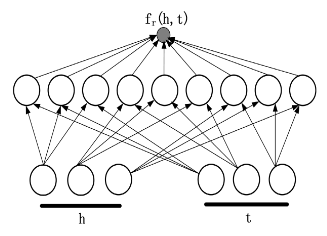
\includegraphics[width=0.45\textwidth]{images/rescal.png}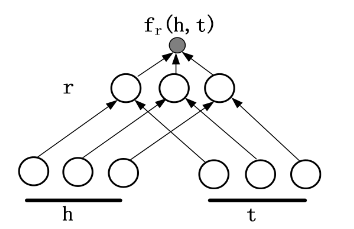
\includegraphics[width=0.45\textwidth]{images/distmult.png}
\caption{RESCAL vs. DistMult}
\label{fig:rescal_distmult}
\end{figure}

Here our dimension size is $D=3$. As we can see in RESCAL this leads to us having $3^2$ latent features for the relation while DistMult requires only $3$.

\subsection{ComplEx}
\label{cha:complex}
While DistMult is more effective in regard to time and space complexity, it can't express antisymmetric relations. RESCAL on the other hand can express this but the size of the relation matrix leads to an explosion in the number of parameters. 
To combine the advantages of both methods Trouillon proposes a model called ComplEx  \cite{trouillon_complex_2016}. ComplEx uses a similar score function as DistMult but instead of calculating the dot product between the embeddings as real numbers, it uses complex vectors to represent the entities and relations. The dot product of complex vectors is referred to as the Hermitian dot product. Other than the dot product of real numbers it is not symmetrical. This enables the model to capture asymmetric relations while retaining the efficiency benefits of DistMult. The score function of ComplEx is 

\begin{equation}
\label{score_complex}
s(h,r,t)=Re(<w_r,e_h,\bar{e}_t>)
\end{equation}

where $e_h, e_t$ and $w_r\in \mathbb{C}$. To use this score function in our loss function, as defined in equation \ref{eq:rescal_loss}, the resulting scores need to be purely real. Therefore after calculating the Hermitian dot product only the real part is kept.  

\subsection{ConvE}
\label{cha:conve}

\section{Comparison of the Approaches}
\label{cha:compare_approaches}

\section{Model Evaluation}
\label{cha:evaluation}